%\newpage
%
%Στην παρούσα εργασία οι όροι κρυπτογραφικό σχήμα, κρυπτοσύστημα χρησιμοποιούνται ως συνώνυμες, σε αντίθεση με τον όρο κρυπτογραφικό κατασκεύασμα που χρησιμοποιείται κυρίως για να αναφερθούμε σε παλαιότερους τρόπους κρυπτογράφησης που χρησιμοποιούνταν στην αρχαιότητα και βασίζονταν κυρίως σε κατασκευαστικούς μηχανισμούς.

\chapter{Εισαγωγή}

\label{chapter:intro}

Στα πλαίσια αυτής της διπλωματικής εργασίας κάνουμε μια μελέτη στις βασικές έννοιες της Κρυπτογραφίας, Αποδείξιμης Ασφάλειας και του Ασφαλούς και Επαληθεύσιμου Υπολογισμού, κυρίως μέσω των πρωτοκόλλων Ασφαλούς Υπολογισμού Πολλών Μερών. Θα μελετήσουμε δηλαδή τα βασικά συστατικά στοιχεία που χρειάζονται στην κατασκευή και στην απόδειξη της ασφάλειας ενός πρωτοκόλλου αυτού του είδους. Μελετάτε ένα ευρύ φάσμα αυτών των πρωτοκόλλων, ξεκινώντας από τα πρώτα πρωτόκολλα που προτάθηκαν στη βιβλιογραφία φτάνοντας μέχρι και τα πιο σύγχρονα. Τέλος, παρουσιάζεται μια Ασφαλούς Υπολογισμού Δύο Μερών BLAS Level-1 βιβλιοθήκης, η οποία κατά τη γνώση μας, παρουσιάζεται πρώτη φορά στη βιβλιογραφία, και χρησιμοποιεί κρυπτογραφικά εργαλεία και έννοιες που θα αναλύσουμε στη συνέχεια.


\section{Κρυπτογραφία}

Η λέξη κρυπτογραφία προέρχεται από τη σύνθεση δύο ελληνικών λέξεων, 'κρύπτο' που σημαίνει μυστικό και 'γράφω'.

\subsection{Ιστορική αναδρομή}

Από την αρχαιότητα κιόλας, υπήρχε η ανάγκη για ασφαλή ανταλλαγή μηνυμάτων. Έτσι, σε πολλούς αρχαίους πολιτισμούς έχει παρατηρηθεί ότι χρησιμοποιούνταν πρωταρχικά κρυπτογραφικά κατασκευάσματα, όπως αυτά της Σκυτάλης \cite{doi:10.1080/0161-119891886902} και του Καίσαρα \cite{9452465}. Ύστερα, παράλληλα με την πρόοδο των μαθηματικών, παρατηρούνται να εμφανίζονται όλο και πιο σύνθετα κρυπτογραφικά κατασκευάσματα βασισμένα στα αυτά. Ιστορικά, η κρυπτογραφία στον πόλεμο αποτελούσε μια μορφής όπλο, ο αντιμαχόμενος που είχε το ισχυρότερο σύστημα ή αυτός που μπορούσε να παραβιάσει την ασφάλεια του συστήματος του αντιπάλου, είχε πρόσβαση σε πληροφορίες που το εξασφάλιζαν σημαντικό πλεονέκτημα. Όπως και στην περίπτωση του πολεμικού εξοπλισμού, άρχισε να εμφανίζεται ανταγωνισμός (arms race) μεταξύ των κρυπτογραφικών κατασκευασμάτων \cite{osti_1671059}. Ιστορικά, το πιο γνωστό τέτοιο παράδειγμα είναι η μηχανή Enigma που χρησιμοποιούσαν οι Γερμανοί στον 2ο Π.Π. την οποία οι Συμμαχικές Δυνάμεις, με τη βοήθεια του Άλαν Τούρινγκ και τον συνάδελφων του, κατάφεραν να παραβιάσουν και να αποκτήσουν σοβαρό πλεονέκτημα στον πόλεμο. Έτσι, παράλληλα με την κρυπτογραφία, αλλά κυρίως από τότε που άρχισε να παίρνει πιο μαθηματική διατύπωση, αναπτύσσεται και ο κλάδος της κρυπτανάλυσης. Η κρυπτανάλυση, στην πιο απλή της μορφή, πρόκειται για την ανάλυση ενός κρυπτοσυστήματος, δίχως πρόσβαση στην κρυφή πληροφορία, συνήθως με τη μορφή κλειδιού, που επιτρέπει αποτελεσματικά την αποκωδικοποίηση του κρυπτοκειμένου, με σκοπό την παραβίαση του και την απόκτηση του απλού κειμένου \cite{Bauer2011}. Οι έννοιες κρυπτογραφικό κλειδί και κρυπτοκείμενο θα οριστούν στην επόμενη ενότητα. Η κρυπτογραφία και η κρυπτανάλυση εντάσσονται στον ευρύτερο κλάδο της κρυπτολογίας.

\subsection{Σύγχρονη Κρυπτογραφία}
Ο κλάδος άρχισε γνωρίζει μεγάλη άνθηση από τότε που οι άνθρωποι άρχισαν να χρησιμοποιούν, μαζικά, τηλεπικοινωνιακά συστήματα για να επικοινωνούν σε μεγάλες αποστάσεις, δηλαδή στις αρχές του 20ού αιώνα, αλλά και πιο συγκεκριμένα όταν η πληροφορία που μετέφεραν άρχισε να γίνεται απόρρητη και να αποκτά μεγάλη αξία, δηλαδή με την έλευση του 2ου Π.Π. Τα πρώτα θεμέλια της μαθηματικής κρυπτογραφίας μπήκαν από τις επιστημονικές εργασίες του Kerchoffs \cite{kerckhoffs1883cryptographie} το 1883 και του Shannon \cite{shannon1945mathematical} το 1949. Στην πρώτη, ο Kerchoffs έθεσε τις βασικές σχεδιαστικές αρχές που πρέπει να διέπουν ένα κρυπτογραφικό σχήμα, μεταξύ των οποίων την πασίγνωστη σχεδιαστική αρχή κατά την οποία η ασφάλεια ενός σχήματος πρέπει να έγκειται μόνο στη μυστικότητα του κλειδιού και να μην εξαρτάται από τη μυστικότητα του αλγορίθμου κρυπτογράφησης. Στην δεύτερη, η κρυπτογραφία μετατρέπεται σε αυστηρό επιστημονικό πεδίο, όπου ορίζεται η έννοια του κρυπτοσυστήματος και η απόλυτη ασφάλεια. Ιστορικά, να αναφέρουμε πως όλα τα κρυπτογραφικά κατασκευάσματα μέχρι τα μέσα του 20ου αιώνα, που άρχισαν να γνωρίζουν άνθηση οι υπολογιστές, κατατάσσονται στην εποχή της Κλασσικής Κρυπτογραφίας, από εκεί και έπειτα που άρχισε να διατυπώνεται με αυστηρό μαθηματικό τρόπο ξεκινάει η εποχή της Σύγχρονης Κρυπτογραφίας. Επαναστατικές ήταν επίσης και οι εργασίες των Diffi-Hellman \cite{10.1109/TIT.1976.1055638} το 1976 και των Rivest, Shamir, Adleman το 1977 \cite{10.1145/359340.359342}, η οποίες ξεκίνησαν την επανάσταση της κρυπτογραφίας δημόσιου κλειδιού. Στην πρώτη θέτονται τα θεμέλια της κρυπτογραφίας δημόσιου κλειδιού και παρουσιάζεται το πρώτο πρωτόκολλο ανταλλαγής κλειδιών, το οποίο χρησιμοποιείται μέχρι και σήμερα και είναι γνωστό στην βιβλιογραφία με τα ονόματα των συγγραφέων της εργασίας, το Πρωτόκολλο Diffie-Hellman (DH) ή αλλιώς το Πρωτόκολλο Ανταλλαγής Κλειδιών Diffie-Hellman (Diffie Hellman Key Exchange ή DHKE). Ωστόσο, στην εργασία αυτή δεν παρουσιάζεται κάποιο κρυπτογραφικό σχήμα δημοσίου κλειδιού με υποστήριξη ανταλλαγής μηνυμάτων ή ψηφιακών υπογραφών. Αυτό παρουσιάστηκε για πρώτη φορά στη δεύτερη εργασία και είναι το πρώτο ιδιαίτερα επιτυχημένο κρυπτοσύστημα δημόσιου κλειδιού, το RSA, που χρησιμοποιείται με παραλλαγές μέχρι και σήμερα. Το κρυπτοσύστημα αυτό αναπτύχθηκε παράλληλα, το 1973, από τον Clifford Cocks όταν δούλευε για το GCHQ, ωστόσο έγινε δημόσια διαθέσιμο (declassified) το 1997.

\subsection{Η κρυπτογραφία σήμερα}
Σήμερα, βρισκόμαστε στην εποχή της 4ης Βιομηχανικής Επανάστασης \cite{drath2014industrie} \cite{skilton20184th}, το διαδίκτυο πλέον αριθμεί αρκετά δισεκατομμύρια συσκευές και καθημερινά παράγονται και αποθηκεύονται αρκετά μεγαλύτερες τάξεις μεγέθους από bytes δεδομένων. Οι εφαρμογές τις κρυπτογραφίας έχουν πλέον ξεφύγει από τους καθαρά πολεμικούς σκοπούς του παρελθόντος, οι οποίοι συνεχίζουν ωστόσο να είναι τα μεγαλύτερα κίνητρα, και έχουν πάρει μια πιο κοινωνικοποιημένη μορφή. Βρίσκονται πλέον σιωπηρά στην καθημερινότητα κάθε ανθρώπου. Η κρυπτογραφία αποτελεί πλέον επιστημονικό κλάδο με πολύ ισχυρά θεμέλια. Το φάσμα της έχει απλωθεί σε πάρα πολλούς τομείς, όπως της ασφαλούς επικοινωνίας (τηλεπικοινωνίες, εφαρμογές μηνυμάτων κα.), της ασφαλούς πρόσβασης και συναλλαγών (τραπεζικές συναλλαγές, ανέπαφες συναλλαγές κα.), των ηλεκτρονικών ψηφοφοριών (κρατικές ψηφοφορίες κα.), ασφαλών αναθέσιμων υπολογισμών και αποθήκευσης (αναθέσιμοι ασφαλείς cloud υπολογισμοί και αποθήκευση κα.), ενσωματωμένων εφαρμογών (συστήματα ασφαλείας όπως συναγερμοί, έξυπνα αντικείμενα όπως συσκευές οικιακής χρήσης κα.) και αποκεντρωμένων εφαρμογών και νομισματικών συστημάτων, όπως αυτή του κρυπτονομίσματος Bitcoin και του Ethereum. Γίνεται άμεσα αντιληπτή η σύνδεση και η αξιοποίηση της από πολλούς επιστημονικούς και βιομηχανικούς κλάδους. Ωστόσο, αξίζει να αναφέρουμε ότι στα περισσότερα προαναφερθέντα συστήματα η κρυπτογραφία παίζει τον ρόλο του διαφανούς ενδιάμεσου επιπέδου (transparent middle layer).

\section{Ασφαλής Υπολογισμός (Secure Computation)}

\subsection[Αναθέσιμος Υπολογισμός και Αποθήκευση (Outsource Computation and Storage)]{Αναθέσιμος Υπολογισμός και \\ Αποθήκευση (Outsource Computation and Storage)}
Η έννοιες του Αναθέσιμου Υπολογισμού (Outsourced Computation) και της Αναθέσιμης Αποθήκευσης (Outsourced Storage), με την ευρύτερη ονομασία Νέφους (Cloud) ή και με τις ισοδύναμες τους, αυτές του Υπολογισμού σε Νέφος (Cloud Computing) και Αποθήκευσης σε Νέφος (Cloud Storage) αντίστοιχα, γίνονται όλο και πιο διαδεδομένες στις μέρες μας. Πολλές φορές, η χρήση τους προέρχεται από επιτακτική ανάγκη, πέρα από επιλογή. Ας αναλύσουμε πως όμως προέκυψε η ανάγκη για τις δύο αυτές έννοιες Αναθεσιμότητας. Η ανάγκη αυτή προκύπτει, από το ότι ο αριθμός της υπολογιστικής ισχύς και αποθηκευτικής ικανότητας της μέσης συνδεδεμένης συσκευής ανά μονάδα χώρου αυξάνεται πολύ πιο αργά σε σχέση με τον αριθμό τον δεδομένων που παράγει και καλείται επεξεργαστεί. Πιο συγκεκριμένα, η αύξηση που παρατηρείται στην περίπτωση της υπολογιστικής και αποθηκευτικής ισχύος ανά μονάδα χώρου είναι το πολύ γραμμική στη μονάδα του χρόνου, ενώ αντίθετα η αύξηση των παραγομένων δεδομένων είναι τουλάχιστον πολυωνυμική στην ίδια μονάδα χρόνου. Αντιθέτως, ο ρυθμός αύξησης της μέσης ταχύτητας σύνδεσης μιας συσκευής στο διαδίκτυο παρατηρείται να είναι εκθετικός, γεγονός που κάνει τις έννοιες των Αναθέσιμου Υπολογισμού και Αποθήκευσης ιδιαίτερα ελκτικές \cite{aljabre2012cloud} \cite{golightly2022adoption} \cite{chen2016perceived}. Για να υποστηρίξουμε τους παραπάνω ισχυρισμούς, αρκεί να αναλογιστούμε πόσοι από εμάς "Δεν διαθέτουμε χώρο στο κινητό μας τηλέφωνο" και αναγκαζόμαστε να χρησιμοποιήσουμε κάποια εξωτερική υπηρεσία αποθήκευσης νέφους ώστε να αποθηκεύσουμε τα αρχεία μας, και πόσοι επιστημονικοί υπολογισμοί και πειράματα εκτελούνται σε υπηρεσίες Νέφους λόγω του ότι δε διαθέτουμε, ή είναι ασύμφορο να την αποκτήσουμε για τη χρήση μας, την κατάλληλη υλικοτεχνική υποδομή

\subsection[Ασφαλής Αναθέσιμος Υπολογισμός και Αποθήκευση (Secure Outsourced Computation and Storage)]{Ασφαλής Αναθέσιμος Υπολογισμός και Αποθήκευση (Secure \\ Outsourced Computation and Storage)}
Θα εξετάσουμε ένα παράδειγμα, από το Διαδίκτυο των Πραγμάτων, για το πως προκύπτει η ανάγκη για εφαρμογή κρυπτογραφικών μεθόδων στη χρήση του Αναθέσιμου Υπολογισμού και Αποθήκευσης. Πλέον, οι αισθητήρες και οι έξυπνες συσκευές (smart devices) βρίσκονται όλο και περισσότερο μέσα στην καθημερινότητα μας, χωρίς απαραίτητα να μας γίνεται αντιληπτό. Το Διαδίκτυο των Πραγμάτων (Internet of Things ή IoT) αρχίζει να είναι όλο ένα και περισσότερο μέρος της πραγματικότητας \cite{gershenfeld2004internet} \cite{li2015internet} . Έξυπνοι αισθητήρες, συσκευές και μηχανές είναι πλέον μέρος αυτής. Όμως, όπως είδαμε και προηγουμένως, το μεγαλύτερο ποσοστό αυτών των συσκευών είναι ανίκανο να επεξεργαστεί και να αποθηκεύσει τον όγκο των δεδομένων που παράγει. Έτσι οι περισσότερες συσκευές, όπως για παράδειγμα ένα έξυπνο ρολόι (smartwatch), πρέπει να στείλουν τα δεδομένα τους σε τρίτους με την κατάλληλη υπολογιστική ισχύ και αποθηκευτική ικανότητα ώστε να κάνουν τους υπολογισμούς και την αποθήκευση των δεδομένων. Έτσι γεννήθηκε το Cloud computing και storage. Τα δεδομένα όμως μπορεί να είναι προσωπικά ή ευαίσθητα ώστε να μην θέλουμε αυτός ο τρίτος να μπορεί να έχει πρόσβαση στο περιεχόμενο τους για να τα επεξεργαστεί, πόσο μάλλον για να τα αποθηκεύσει. Αυτή η κεντροποίηση (centralization) του υπολογισμού και της αποθήκευσης εναποθέτει την ασφάλεια των δεδομένων σε κάποιον Έμπιστο Τρίτο Μέρος (Trusted Third Party ή TTP). Δυστυχώς, όσο έμπιστος και αν είναι αυτός ο τρίτος, στην πράξη δημιουργείται Μοναδικό Σημείο Αστοχίας (Single Point of Failure) αφού αυτός ο τρίτος καταλήγει να κατέχει πολύτιμη ποσότητα δεδομένων και να γίνεται στόχος κυβερνοεπιθέσεων, το οποίο επαληθεύεται από τις δεκάδες διαρροές δεδομένων (data breaches) που συμβαίνουν πλέον καθημερινά. Έτσι, προκύπτει η ανάγκη για εφαρμογή κρυπτογραφικών μεθόδων με απώτερο σκοπό να περιοριστεί η πρόσβαση στα δεδομένα των χρηστών στις πλέον απαραίτητες οντότητες. Μπορούμε να φανταστούμε ένα σενάριο στο οποίο, κρυπτογραφήσουμε τα δεδομένα πριν τα στείλουμε σε κάποιον τρίτο για επεξεργασία, αυτός να κάνει τον υπολογισμό πάνω στην κρυπτογραφημένη τους μορφή και να μας επιστρέφει τα αποτελέσματα, ή την ανάκτηση αυτών, είτε σε κρυπτογραφημένη μορφή που μόνο εμείς θα έχουμε πρόσβαση, είτε σε απλή (μη κρυπτογραφημένη μορφή), όπου στην περίπτωση αυτή θα είχε πρόσβαση και αυτός ο τρίτος, ανάλογα με το αν το αποτέλεσμα του υπολογισμού το θεωρούμε ευαίσθητο ή όχι. Αντίστοιχα, μπορούμε να σκεφτούμε και παρόμοια σενάρια σχετικά με την αποθήκευση δεδομένων.

Το πρόβλημα που σχετίζεται με την με την Ασφαλή Αποθήκευση (Secure Storage) των δεδομένων, είναι εκ φύσεως πιο εύκολο στην επίλυση του και έχει σε ένα βαθμό επιλυθεί στις μέρες μας, για αυτό και δεν θα αναφερθούμε περαιτέρω σε αυτό στα πλαίσια αυτής της εργασίας. Ο αναγνώστης που ενδιαφέρεται να διαβάσει περισσότερα για αυτό μπορεί να ανατρέξει στις εργασίες \cite{10.1145/1315245.1315318} \cite{DBLP:journals/access/Gupta0LB22}. 

Το πρόβλημα που σχετίζεται με την ασφαλή επεξεργασία των δεδομένων έρχεται να λύσει ο Ασφαλής Υπολογισμός (Secure Computation), που χρησιμοποιείται ως μια γενική έννοια που συμπεριλαμβάνει όλες τις μεθόδους που χρησιμοποιούνται για τον υπολογισμό σε κρυπτογραφημένα δεδομένα. Πέραν όμως του ασφαλούς υπολογισμού, μας ενδιαφέρει και η επαλήθευση των αποτελεσμάτων, δηλαδή η εξακρίβωση αν τα αποτελέσματα όντως προέκυψαν από τον επιθυμητό υπολογισμό, αυτό είναι το αντικείμενο του Επαληθέυσιμου Υπολογισμού (Verifiable Computation). Ο Ασφαλής και ο Επαληθεύσιμος υπολογισμός αποτελούν από τους πιο ενεργούς κλάδους της κρυπτογραφίας σήμερα. Υπάρχουν δύο κύριοι υποκλάδοι που συνδυάζουν και τα δύο αυτά χαρακτηριστικά, ο Ασφαλής Αναθέσιμος Υπολογισμός (Secure Outsourced Computation) και ο Ασφαλής Υπολογισμός Πολλών Μερών (Secure Multi-Party Computation ή (SMPC)\footnote{Πρέπει να αναφέρουμε ότι στην βιβλιογραφία οι όροι Ασφαλής Υπολογισμός Πολλών Μερών (Secure Multi-Party Computation ή  SMPC) και Υπολογισμός Πολλών Μερών (Multi-Party Computation ή MPC)  χρησιμοποιούνται ως ταυτόσημοι, ωστόσο επειδή ο πρώτος είναι πιο περιγραφικός, στα πλαίσια αυτής της εργασίας θα χρησιμοποιήσουμε αυτόν.}. Η κύρια διαφορά του Ασφαλής Υπολογισμού Πολλών Μερών και του Ασφαλή Αναθέσιμου Υπολογισμού είναι ότι ο πρώτος περιλαμβάνει αποκλειστικά μη διαδραστικά (non-interactive) πρωτόκολλα ενώ ο δεύτερος περιλαμβάνει αποκλειστικά διαδραστικά (interactive) πρωτόκολλα.

\subsubsection{Ομομορφική Κρυπτογράφηση (Homomorphic Encryption ή HE)}
Η Ομομορφική Κρυπτογράφηση είναι ένα από τα βασικότερα εργαλεία που χρησιμοποιούνται στην επίτευξη Ασφαλούς Αναθέσιμου Υπολογισμού. Με τον όρο Ομομορφική Κρυπτογράφηση αναφερόμαστε σε μια κλάση μη διαδραστικών κρυπτογραφικών σχημάτων που επιτρέπουν ανάλογα με τη φύση τους, την εφαρμογή μίας ή περισσότερων πράξεων, για μία ή περισσότερες φορές σε ένα κρυπτοκέιμενο. Η έννοια αυτή είναι πολύ στενά συνδεδεμένη με αυτήν της Ευπλαστότητας (Malleability). Παρακάτω ορίζουμε την Ομομορφική Κρυπτογράφηση και τις κύριες κατηγορίες σχημάτων που εντάσσονται σε αυτήν.

\begin{definition}
\textbf{Ομομορφικό Σχήμα Κρυπτογράφησης (\EN{Homomorphic Encryption \\ Scheme} ή \EN{HE Scheme})} : Ένα κρυπτογραφικό σχήμα είναι ομομορφικό σε μια πράξη $\star$ όταν υποστηρίζει την παρακάτω ισοδυναμία
\begin{equation}
E_k(m_1) \star E_k(m_2) = E_k(m_1 \star m_2), \forall m_1, m_2 \in M
\end{equation}
όπου $E$ είναι ο αλγόριθμος κρυπτογράφησης και $M$ ο χώρος των μηνυμάτων.
\end{definition}
%
Διακρίνουμε τις εξής κατηγορίας Ομομορφικής Κρυπτογραφίας :
%
\begin{definition}
\begin{itemize}[leftmargin=*]
\textbf{Κύριες Κατηγορίες Ομομορφικής Κρυπτογράφησης} :
\item \textbf{Μερικώς Ομομορφικό Σχήμα Κρυπτογράφησης (Partially Homomorphic Scheme)} : Επιτρέπει μόνο ένα είδος πράξης χωρίς περιορισμό στον αριθμό των φορών που μπορεί να εφαρμοστεί σε ένα κρυπτοκείμενο.
\item \textbf{Κάπως Ομομορφικό Σχήμα Κρυπτογράφησης (Somewhat Homomorphic Encryption Scheme ή SWHE Scheme)} : Επιτρέπει περιορισμένο αριθμό πράξεων που μπορούν να εφαρμοστούν περιορισμένες φορές σε ένα κρυπτοκείμενο.
\item \textbf{Πλήρες Ομομορφικό Σχήμα Κρυπτογράφησης (\EN{Fully Homomorphic Encryption \\ Scheme} ή \EN{FHE Scheme})} : Δεν έχει περιορισμό ούτε στο πλήθος των πράξεων ούτε στον αριθμό των φορών που μπορούν αυτές να εφαρμοστούν σε ένα κρυπτοκείμενο.
\end{itemize}
\end{definition}

Το 2009 ο Gentry στη διατριβή του \cite{10.1145/1536414.1536440} δημιούργησε το πρώτο Πλήρες Ομομορφικό Κρυπτογραφικό Σχήμα, ένα ανοιχτό πρόβλημα για πάνω από 30 χρόνια στον κλάδο της κρυπτογραφίας. Ωστόσο, παρά την πολλή έντονη ερευνητική δραστηριότητα και τα πολλά κρυπτογραφικά σχήματα που έχουν προταθεί στη βιβλιογραφία, στον κλάδο της Πλήρους Ομομορφικής Κρυπτογραφίας, δεν έχουν βρεθεί ακόμα ιδιαίτερα πρακτικά σχήματα που να μπορούν να χρησιμοποιηθούν αποτελεσματικά στην πράξη. Συνήθως είτε έχουν πολύ μεγάλο μέγεθος κλειδιών είτε η διαδικασία εκκίνησης του πρωτοκόλλου είναι πολύ χρονοβόρα \cite{10.1007/978-3-642-20465-4_9}.

Στο Σχήμα \ref{fig:he_timeline} βλέπουμε την Ιστορική εξέλιξη της Ομομορφικής Κρυπτογραφίας μέχρι την ανακάλυψη του πρώτου Πλήρες Ομομορφικού Κρυπτογραφικού Σχήματος από τον Gentry.

\begin{figure}
    \centering
    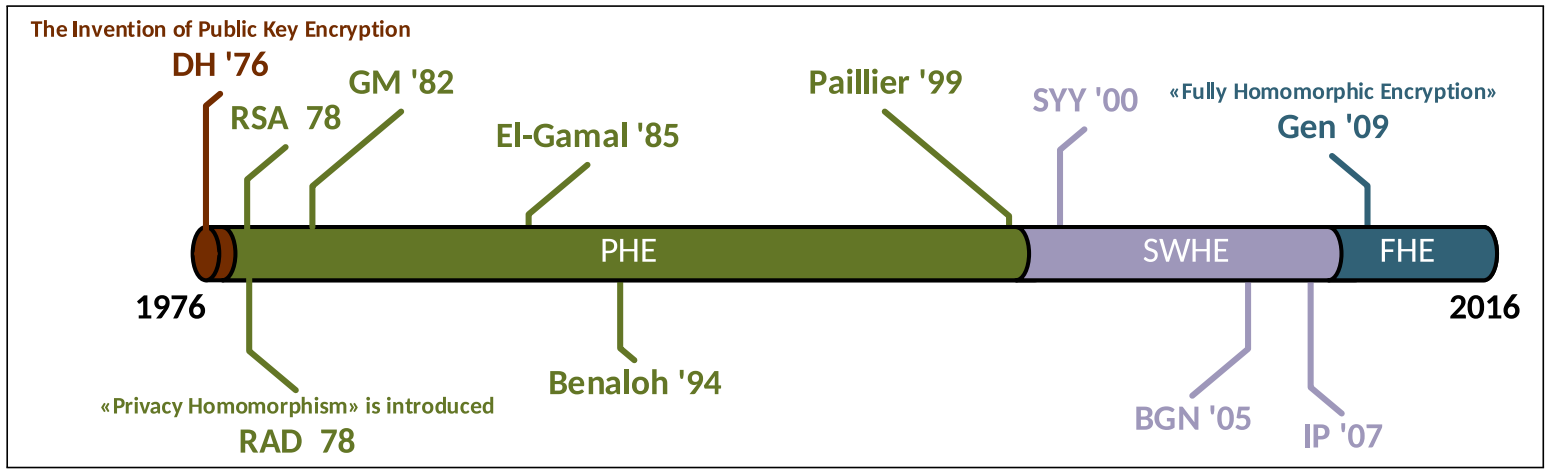
\includegraphics[width=0.8\columnwidth]{./01_body/images/he_timeline.png}
    \caption{Η ιστορική εξέλιξη των Ομομορφικών Σχημάτων μέχρι το πρώτο Πλήρες Ομομορφικό Κρυπτογραφικό Σχήμα \cite{acar2018survey}.}
    \label{fig:he_timeline}
\end{figure}

\subsubsection[Ασφαλής Υπολογισμός Πολλών Μερών (Secure Multi Party Computation ή SMPC)]{Ασφαλής Υπολογισμός Πολλών Μερών (Secure Multi Party \\ Computation ή SMPC)}
Με τον όρο Ασφαλής Υπολογισμών Πολλών Μερών, αναφερόμαστε σε μια κλάση διαδραστικών κρυπτογραφικών σχημάτων η οποία επιτρέπει σε δύο ή περισσότερους συμμετέχοντες που διαθέτουν αντίστοιχες εισόδους (ο κάθε συμμετέχον μπορεί να έχει παραπάνω από μία είσοδο, για χάριν απλότητας όμως μπορούμε να τις θεωρήσουμε ως μια, η οποία μπορεί να ενσωματώνει περισσότερες από μία μέσω κάποιας δομής όπως μια λίστα ή ένα διατεταγμένος ζεύγος), αλλά δεν εμπιστεύονται ο ένας τον άλλον, να υπολογίσουν τις εξόδους μιας συνάρτησης εισάγοντας δημόσια τις από εισόδους τους και εκτελώντας κάποιο κατανεμημένο, ή και μη, πρωτόκολλο. Ο στόχος ενός SMPC πρωτοκόλλου είναι να υπολογίσει σωστά τη συνάρτηση με βάση την είσοδο του κάθε συμμετέχον και να αποκρύψει από κάθε συμμετέχον οποιαδήποτε πληροφορία σχετικά με την είσοδο κάποιου άλλου συμμετέχοντος. Στην περίπτωσή των δύο συμμετεχόντων, αναφερόμαστε ως Ασφαλής Υπολογισμών Δύο Μερών (Secure Two Party Computation ή 2PC). Ο Ασφαλής Υπολογισμός Πολλών Μερών ορίζεται ως εξής :

\begin{definition}
\textbf[Ασφαλής Υπολογισμός Πολλών Μερών (Secure Multi Party Computation ή SMPC)]{Ασφαλής Υπολογισμός Πολλών Μερών (Secure Multi Party Computation ή SMPC)} : Είναι μια κλάση διαδραστικών κρυπτογραφικών σχημάτων που επιτρέπουν σε συμμετέχοντες $P_1, P_2, \dots, P_n$ με αντίστοιχες εισόδους $x_1, x_2, \dots, x_n$ να υπολογίσουν την συνάρτηση την έξοδο $y$ της συνάρτησης $f$, ως $y = f(x_1, x_2, \dots, x_n)$ και ικανοποιούν τις παρακάτω ιδιότητες :

\begin{itemize}
    \item \textbf{Ορθότητα} : Η έξοδος $y$ είναι η σωστή έξοδος της συνάρτησης για τις δεδομένες εισόδους $x_1, x_2, \dots, x_n$
    \item \textbf{Ιδιωτικότητα} : Η έξοδος $y$ είναι η μόνη πληροφορία που φανερώνει το πρωτόκολλο.
\end{itemize}
\end{definition}

Το πρώτο πρωτόκολλο για SMPC παρουσιάστηκε από τον Yao το 1986 στις εργασίες \cite{4568207} \cite{4568388} και προτάθηκε ως πρωτόκολλο επίλυσης του Προβλήματος των Εκατομμυριούχων (\EN{Millionaires' Problem}). Στην βιβλιογραφία σήμερα αναφέρεται ως Μπερδεμένα Δίκτυα Yao (\EN{Yao's Garbled Circuits} ή \EN{Yao's-GC} ή YaoGC). Θα αναλύσουμε το πρωτόκολλο αυτό καθώς και άλλα πρωτόκολλα για SMPC στην Ενότητα \ref{chapter:SMPC}.